%UNIT 10: SPRING MASS SYSTEM AND LINEAR SYSTEMS
%%%%%%%%%%%%%%%%%%%%%%%%%%%
%%%% Put the following at the top of each .tex file  %
\pagestyle{fancy}
\renewcommand{\theUnit}{5.4 and 9.5}
\ifthenelse{\isundefined{\UnitPageNumbers}}{}{\setcounter{page}{1}}
\rhead{Section \theUnit: Stability of Equilibrium Solutions}
\lhead{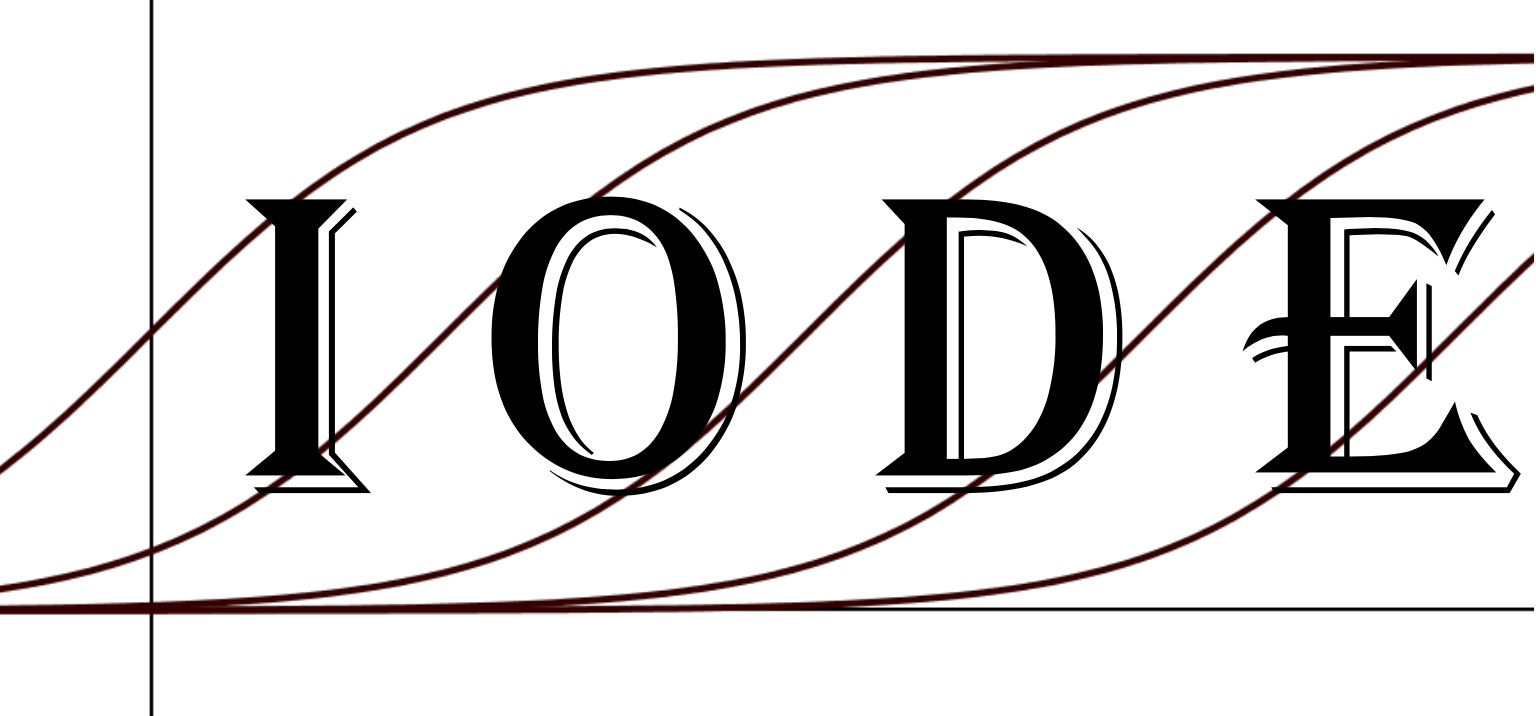
\includegraphics[width=1.25cm]{IODE-logo.png}}
\rfoot{\mypage}
\lfoot{}
\cfoot{}
\fancypagestyle{firstfooter}{\footskip = 50pt}
\renewcommand{\footrulewidth}{.4pt}
%%%%%%%%%%%%%%%%%%%%%%%%%%%
\vspace*{-20pt} \thispagestyle{firstfooter}
\pagebegin{Stability: Long Run Behavior of Solutions}

Recall model of the bacteria populations in Colony 1 and Colony 2 given by system of differential equations \label{13problem3}
\begin{align*}
\frac{dx}{dt} &= 3x+10y \\
\frac{dy}{dt} &= -2y
\end{align*}

We previously found the general solution for this system, which can be expressed as

\begin{align*}
x(t)&= C_1e^{3t} + C_2 e^{-2t} \\
y(t)&= - \frac{1}{2} C_2 e^{-2t} \\
\end{align*}

\bb
\ii Give the solutions if in addition we have the initial condition $(x(0),y(0))= (3,0)$.\label{14problem1}

\vfill

\ii Give the solutions if in addition we have the initial condition $(x(0),y(0))= (2,-1)$.\label{14problem2}

\vfill

\ii Sketch the graphs (in the phase plane) of the solution with initial condition $(x(0),y(0))= (3,0)$ and the solution with initial condition $(x(0),y(0))= (2,-1)$.\label{14problem3}

\vfill \vspace{2in}

\ii Using your graph in problem \ref{14problem3}, make a rough sketch of the solution corresponding to the initial conditions $(x(0),y(0))= (1,1)$ and $(x(0),y(0))= (1,-1)$.\label{14problem4}

\ee

\clearpage
\pagebegin{Eigenvectors}
For the system 

\[ \left[ \begin{array}{c} x' \\ y' \end{array} \right] =
\left[ \begin{array}{cc} 3 & 10 \\ 0 & -2 \end{array} \right]
\left[ \begin{array}{c} x\\ y \end{array} \right], \]

$\mathbf{v}_1=\langle 3, 0 \rangle$ is an \textbf{eigenvector} corresponding to the eigenvalue $r_1 = 3$ and $\mathbf{v}_2=\langle -2, 1 \rangle$ is an eigenvector of $r_2=-2$. From phase plane graph in problem \ref{14problem4}, we see that any solution that starts on the line passing through the eigenvector:
\bi
\ii $\mathbf{v}_1=\langle 3, 0 \rangle$ points directly away from the equilibrium at the origin.
\ii $\mathbf{v}_2=\langle 2, -1 \rangle$ points directly towards the origin.
\ii The sign of the eigenvalue determines whether solutions move towards or away from the equilibrium.
\ei

Using the eigenvectors we can express the solutions in vector form:
\[  \left[ \begin{array}{c} x(t) \\ y(t) \end{array} \right] =
\left[ \begin{array}{rl}
C_1e^{3t}+&C_2e^{-2t}  \\
 &- \frac{1}{2}C_2e^{-2t}
\end{array} \right]  =
C_1e^{r_1t} \mathbf{v}_1+ C_2 e^{r_2t} \mathbf{v}_2. \]

In general, $\mathbf{v}$ is an \textbf{eigenvector} for the eigenvalue $\lambda$ of a square matrix $\mathbf{A}$ if and only if
\[ \mathbf{A} \mathbf{v} = \lambda \mathbf{v}. \]

\clearpage
\pagebegin{Vector Form of Solutions}

\bb[resume]
\ii Consider the system of differential equations:

%%%%%%%%%%%%
%% this has solution
%%   $\lambda =7$ has an eigenvector $\dsty \v_1= \left[ \begin{array}{c} 1 \\ 2 \end{array} \right]$, and 
%%   $\lambda =-2$ has an eigenvector $\dsty \v_2= \left[ \begin{array}{c} 1 \\ -2/3 \end{array} \right]$.
%%%%%%%

\[ \left[ \begin{array}{c}
x'\\
y'
\end{array} \right] = 
\left[ \begin{array}{cc}
1 & 3 \\
4 & 5 
\end{array} \right]
\left[ \begin{array}{c}
x\\
y
\end{array} \right] \]
Find the eigenvalues and eigenvectors for the system and give the general solution in vector form. Then make a sketch of several solutions to this system in the phase plane. \label{14problem5} 


\clearpage

\pagebegin{Eigenvalues and Solutions in the Phase Plane}

\ii Match the vector fields labeled A-F (on the next page) with a system of differential equations whose matrix of coefficients has the given eigenvalues.\label{14problem6} 

\bs

\begin{center}\begin{tabular}{|l|l|}
\hline
Eigenvalues of matrix of coefficients & Label of corresponding phase plane\\
\hline
 & \\
$\lambda_1  = 4$ and $\lambda_2=1$ & \\ % B
& \\
\hline
& \\
$\lambda_1 = -4$ and $\lambda_2 = -2$ & \\ % C
& \\
\hline
& \\
$\lambda = 9$ (repeated) & \\ % F
& \\
\hline
& \\
$\lambda = \pm 2i$ & \\ % A
%actual graph is \pm i
& \\
\hline
& \\
$\lambda = 3 \pm 2i$  & \\ % E
& \\
\hline
& \\
$\lambda = -3 \pm 2i$  & \\ % D
%actual graph is -2 \pm i \sqrt{6} 
& \\
\hline
\end{tabular}\end{center}

\clearpage

\hspace{-0.7in} \begin{tabular}{|c|c|}
\hline
A. 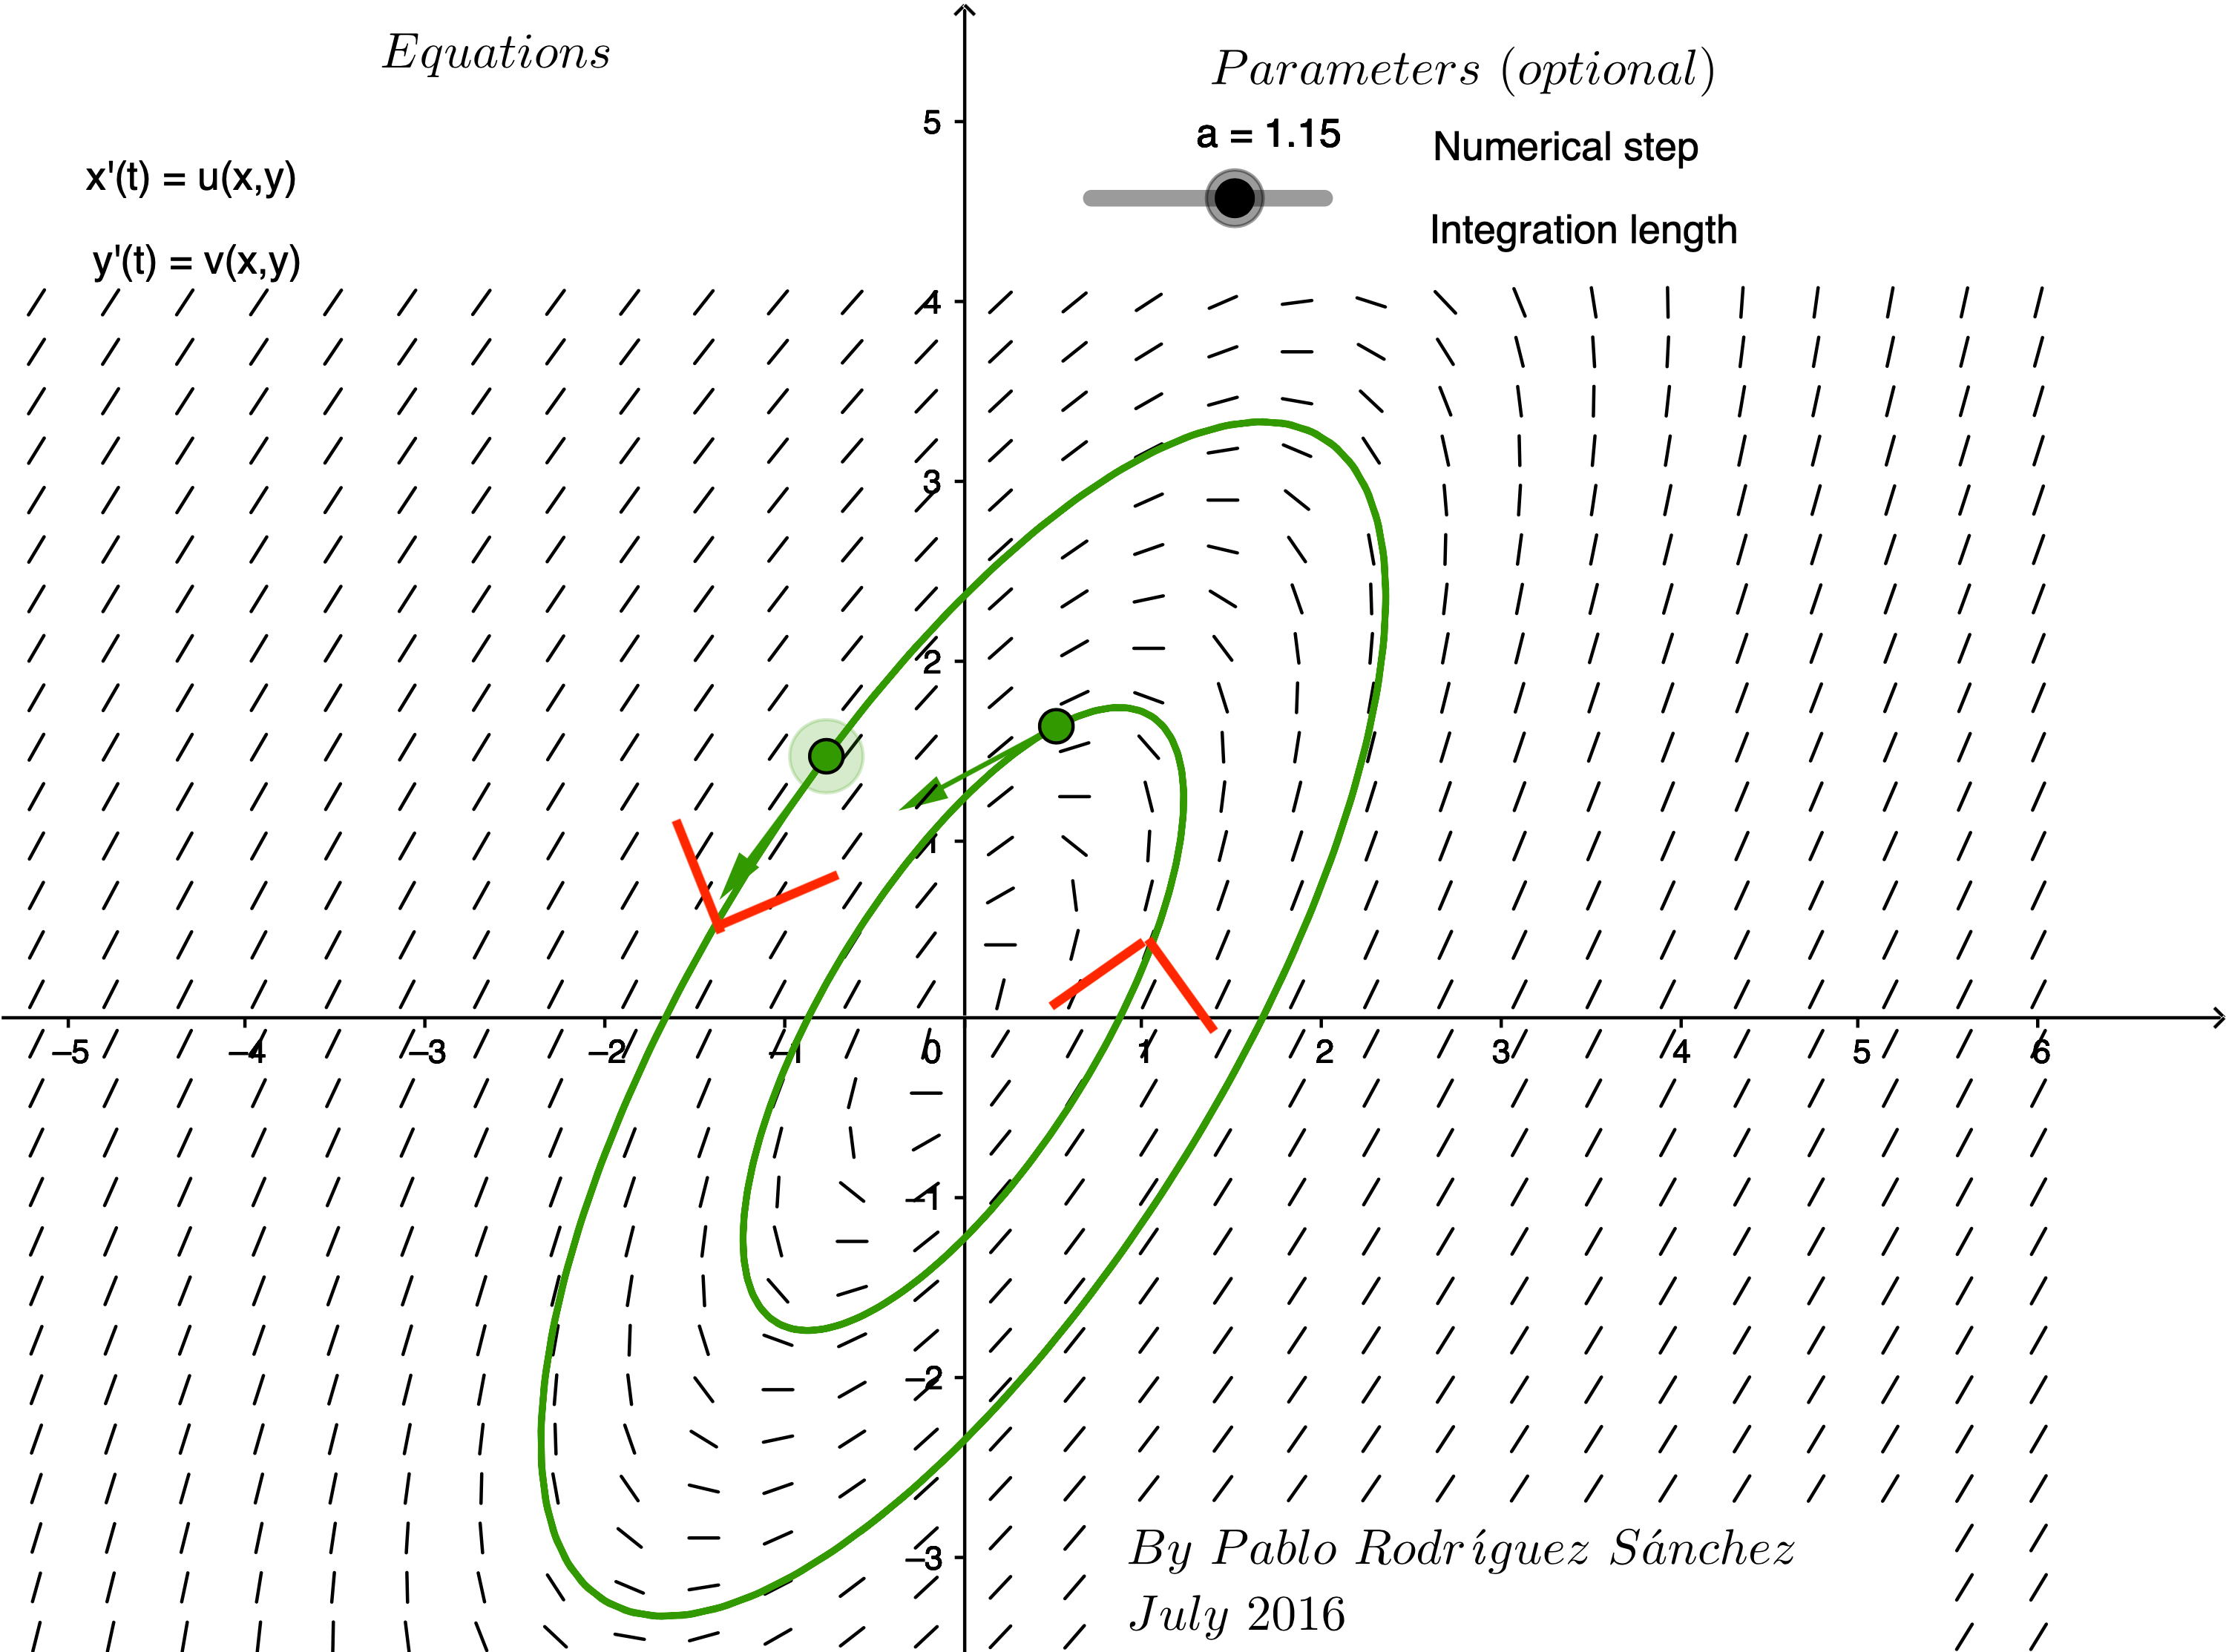
\includegraphics[width=0.45\tw]{14/14-pure-imag.png} &
B. 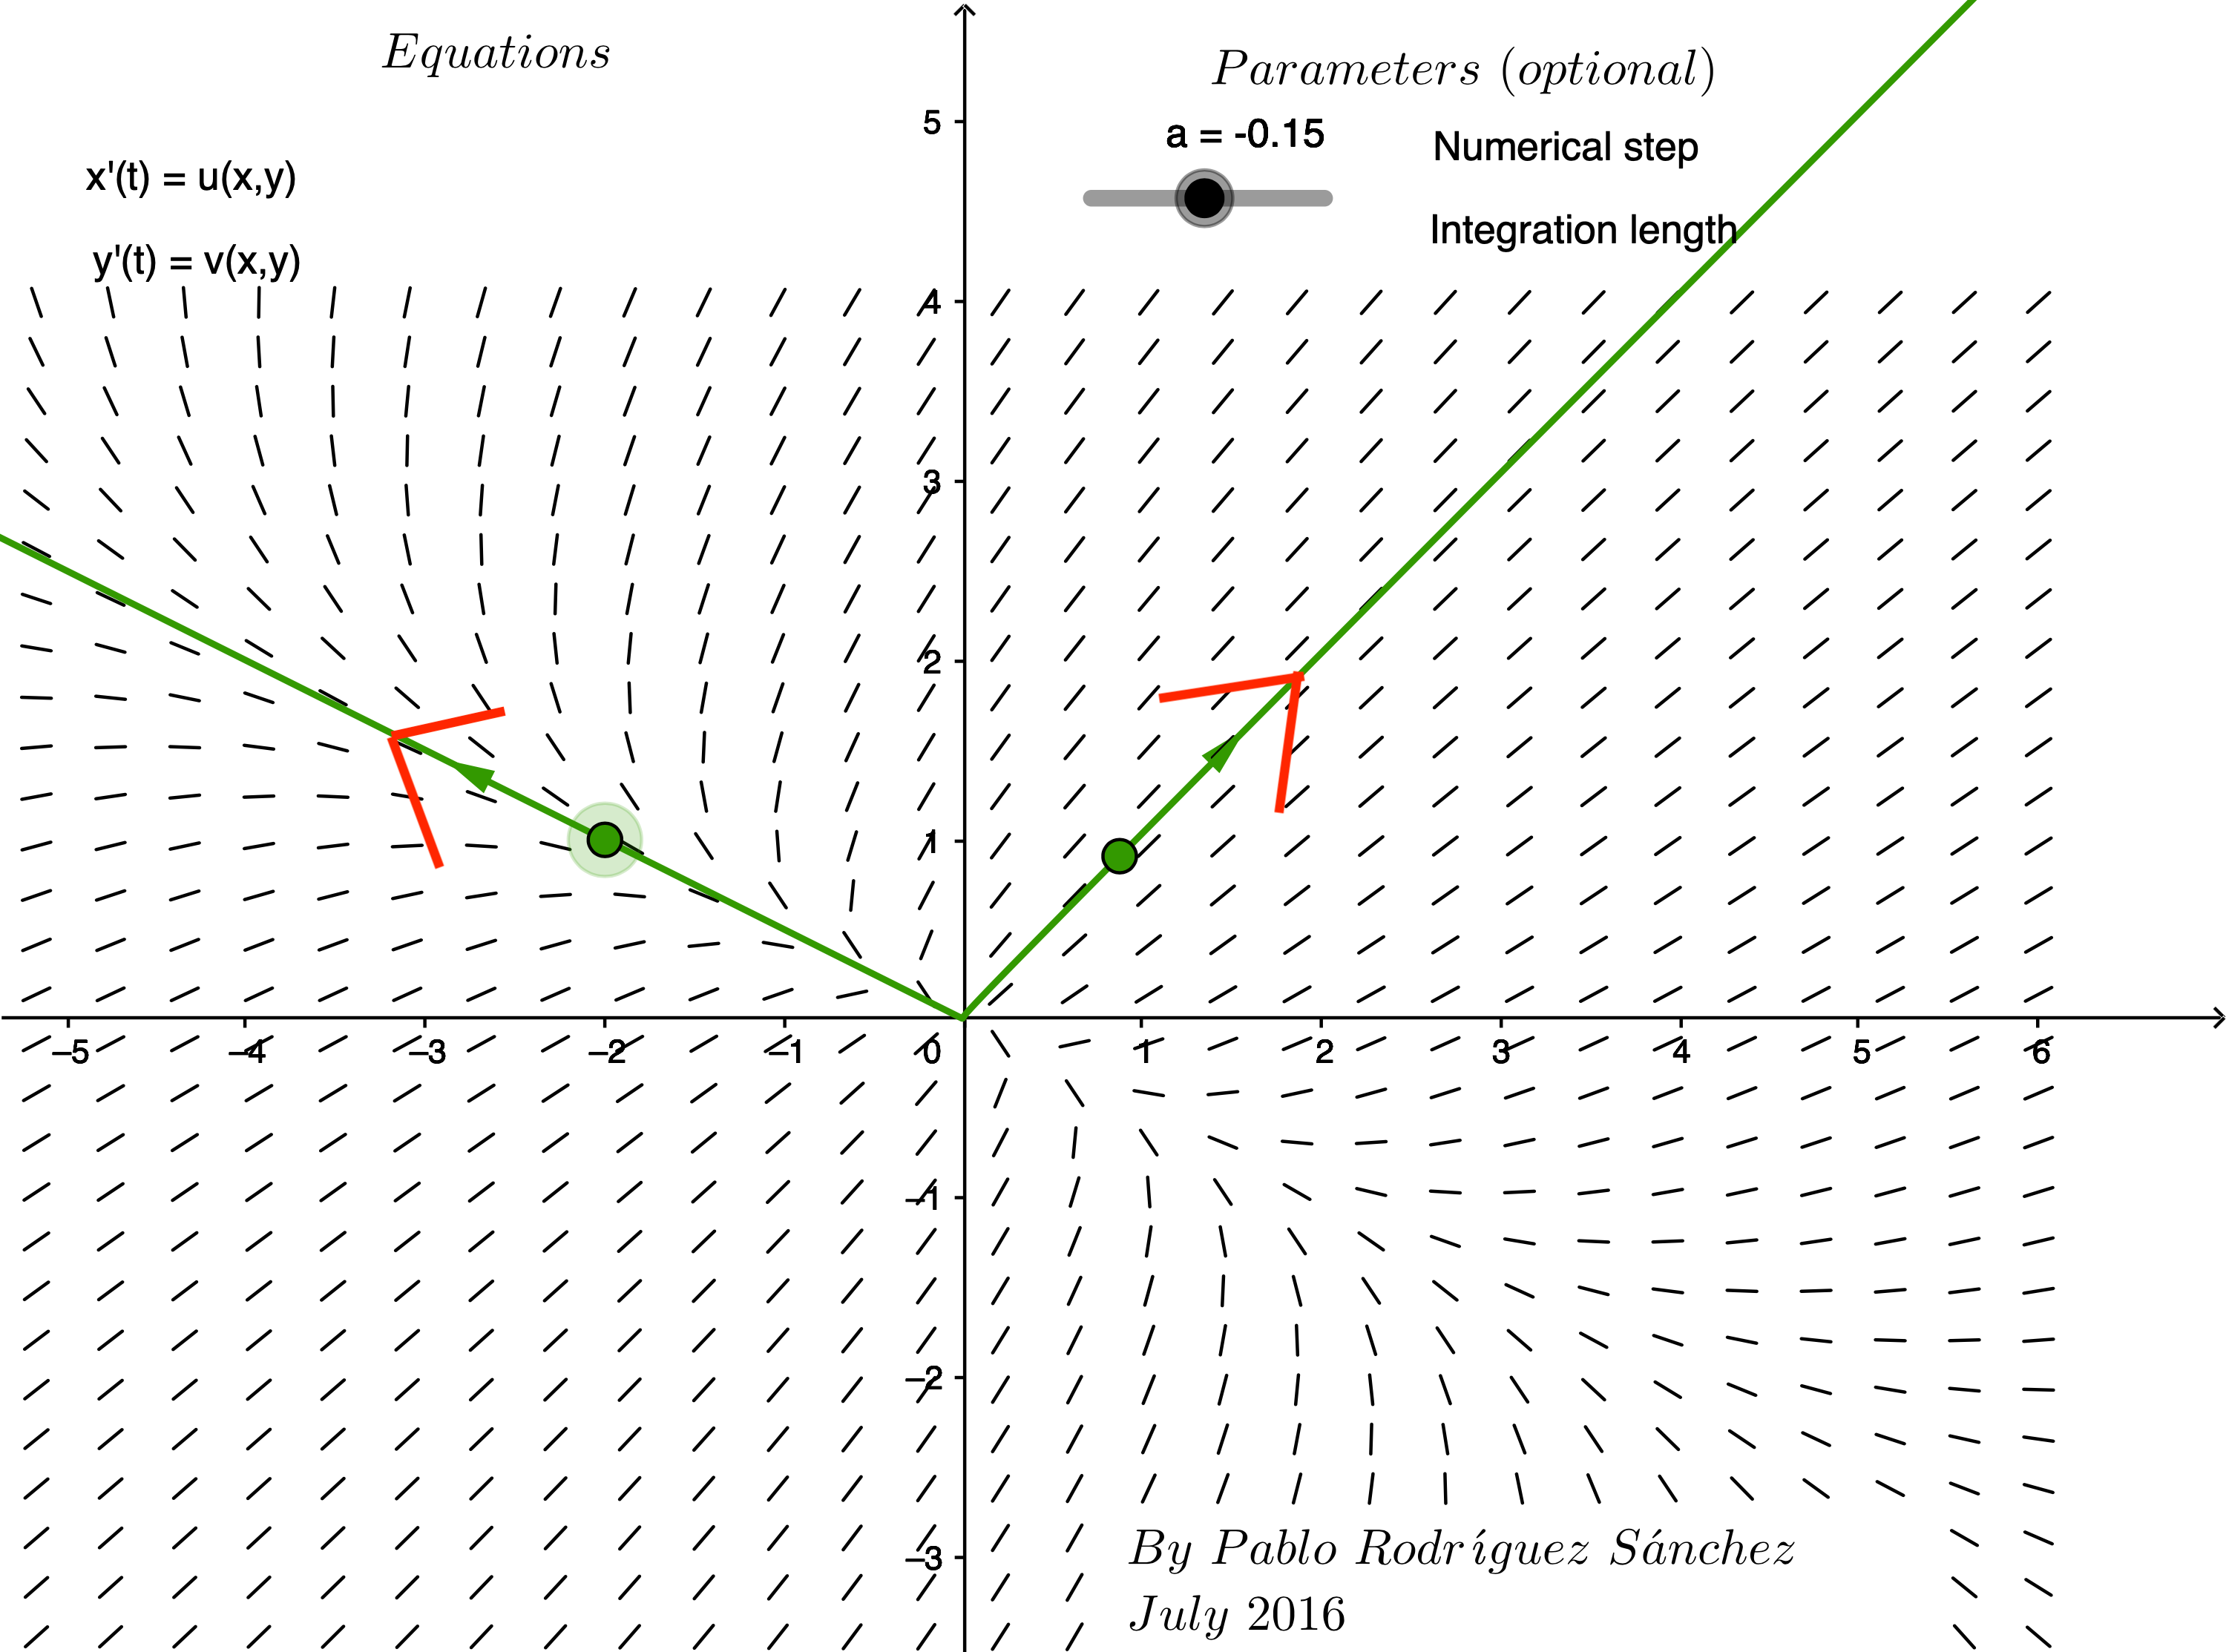
\includegraphics[width=0.45\tw]{14/14-distinct-positive.png} \\
\hline
C. 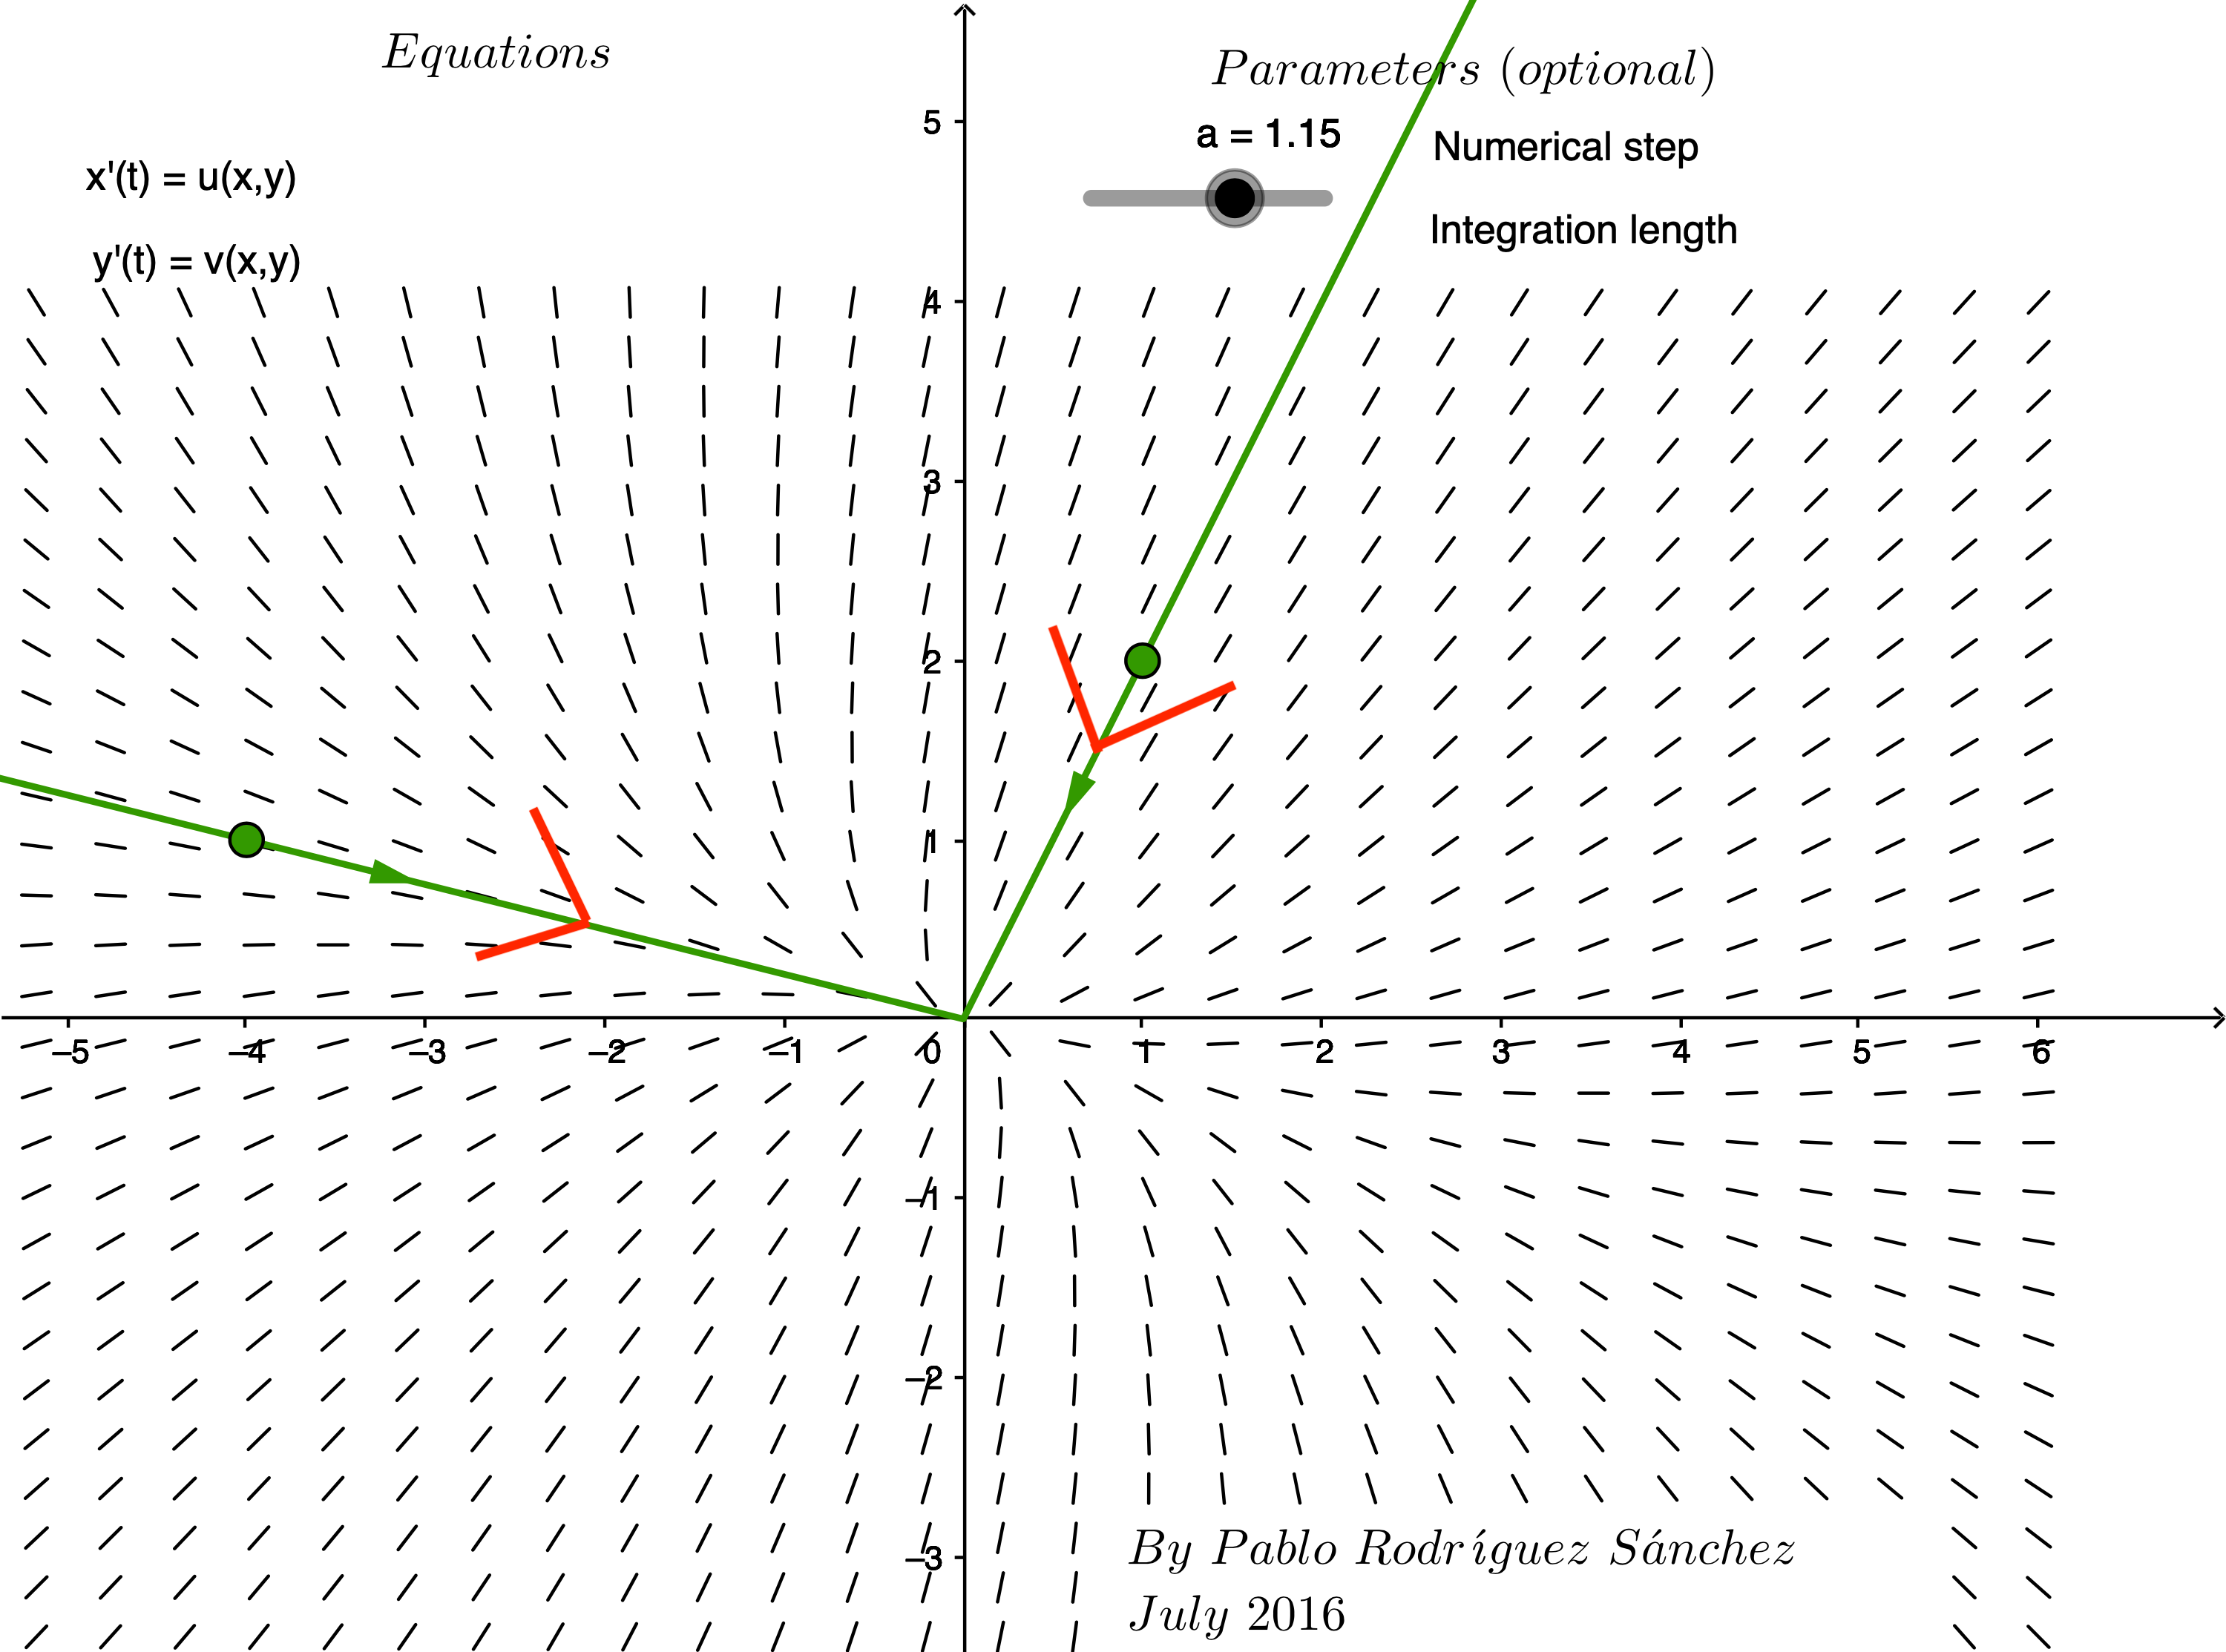
\includegraphics[width=0.45\tw]{14/14-distinct-neg.png} &
D. 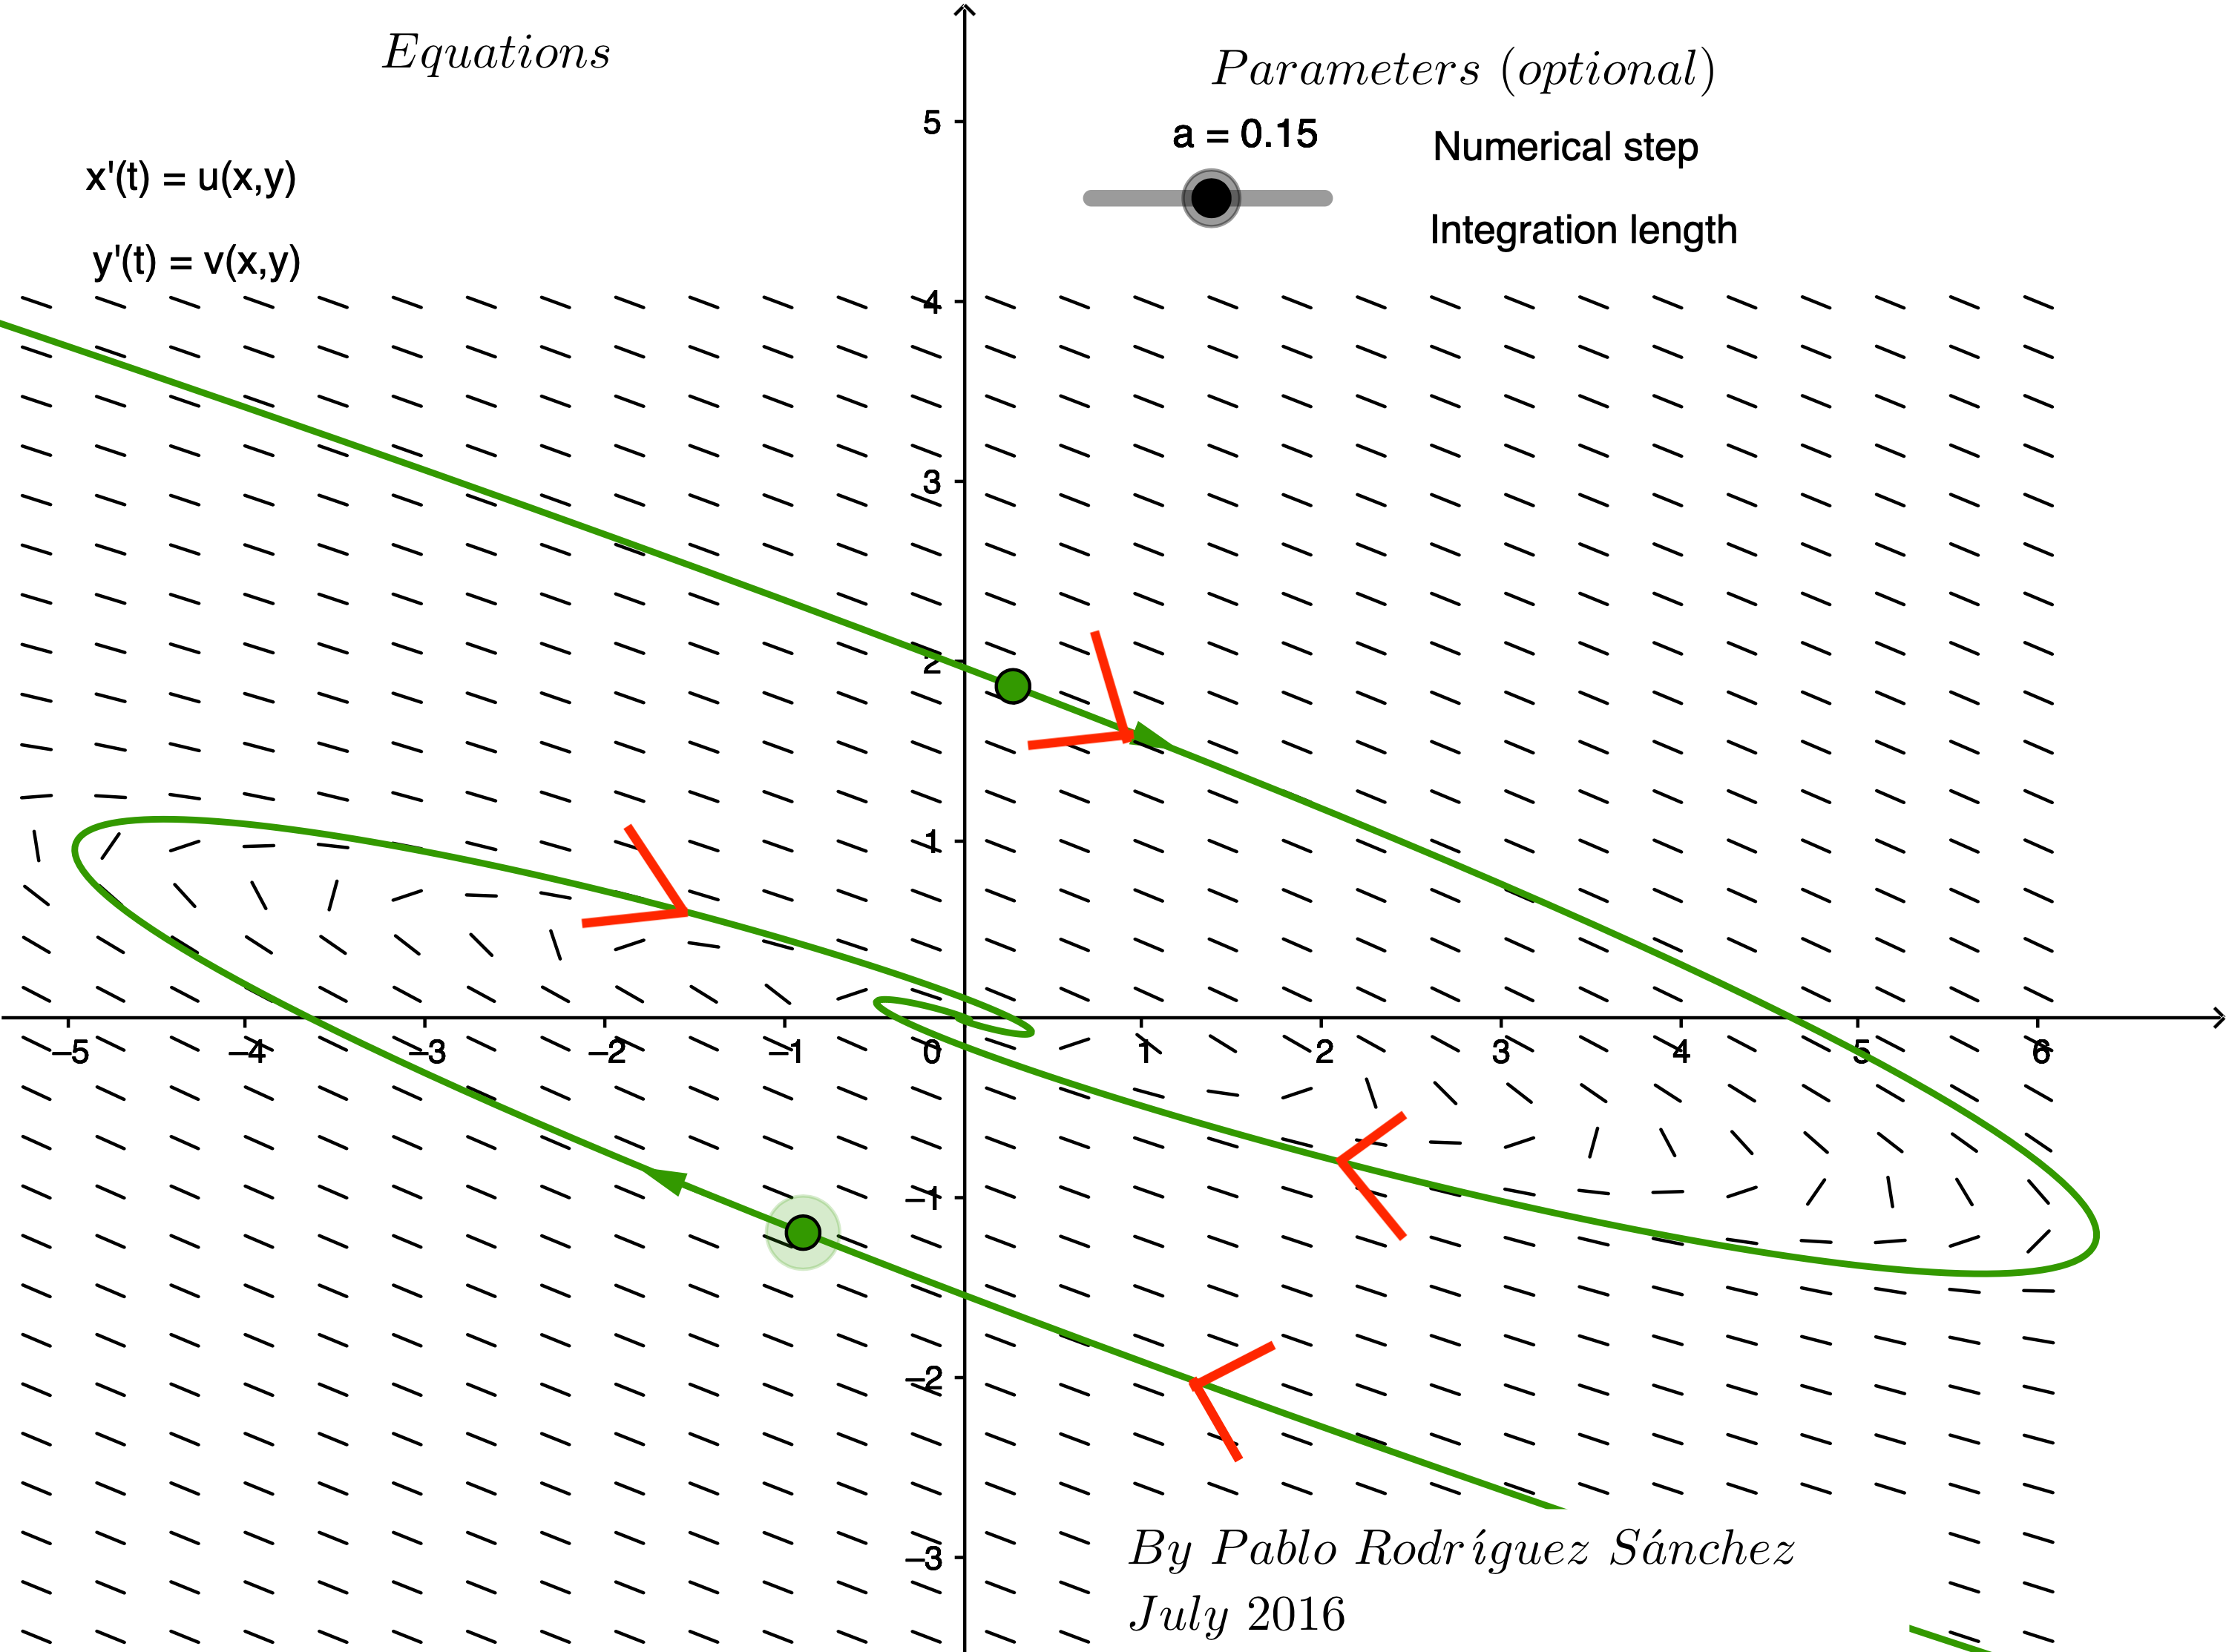
\includegraphics[width=0.45\tw]{14/14-complex-neg.png} \\
\hline
E. 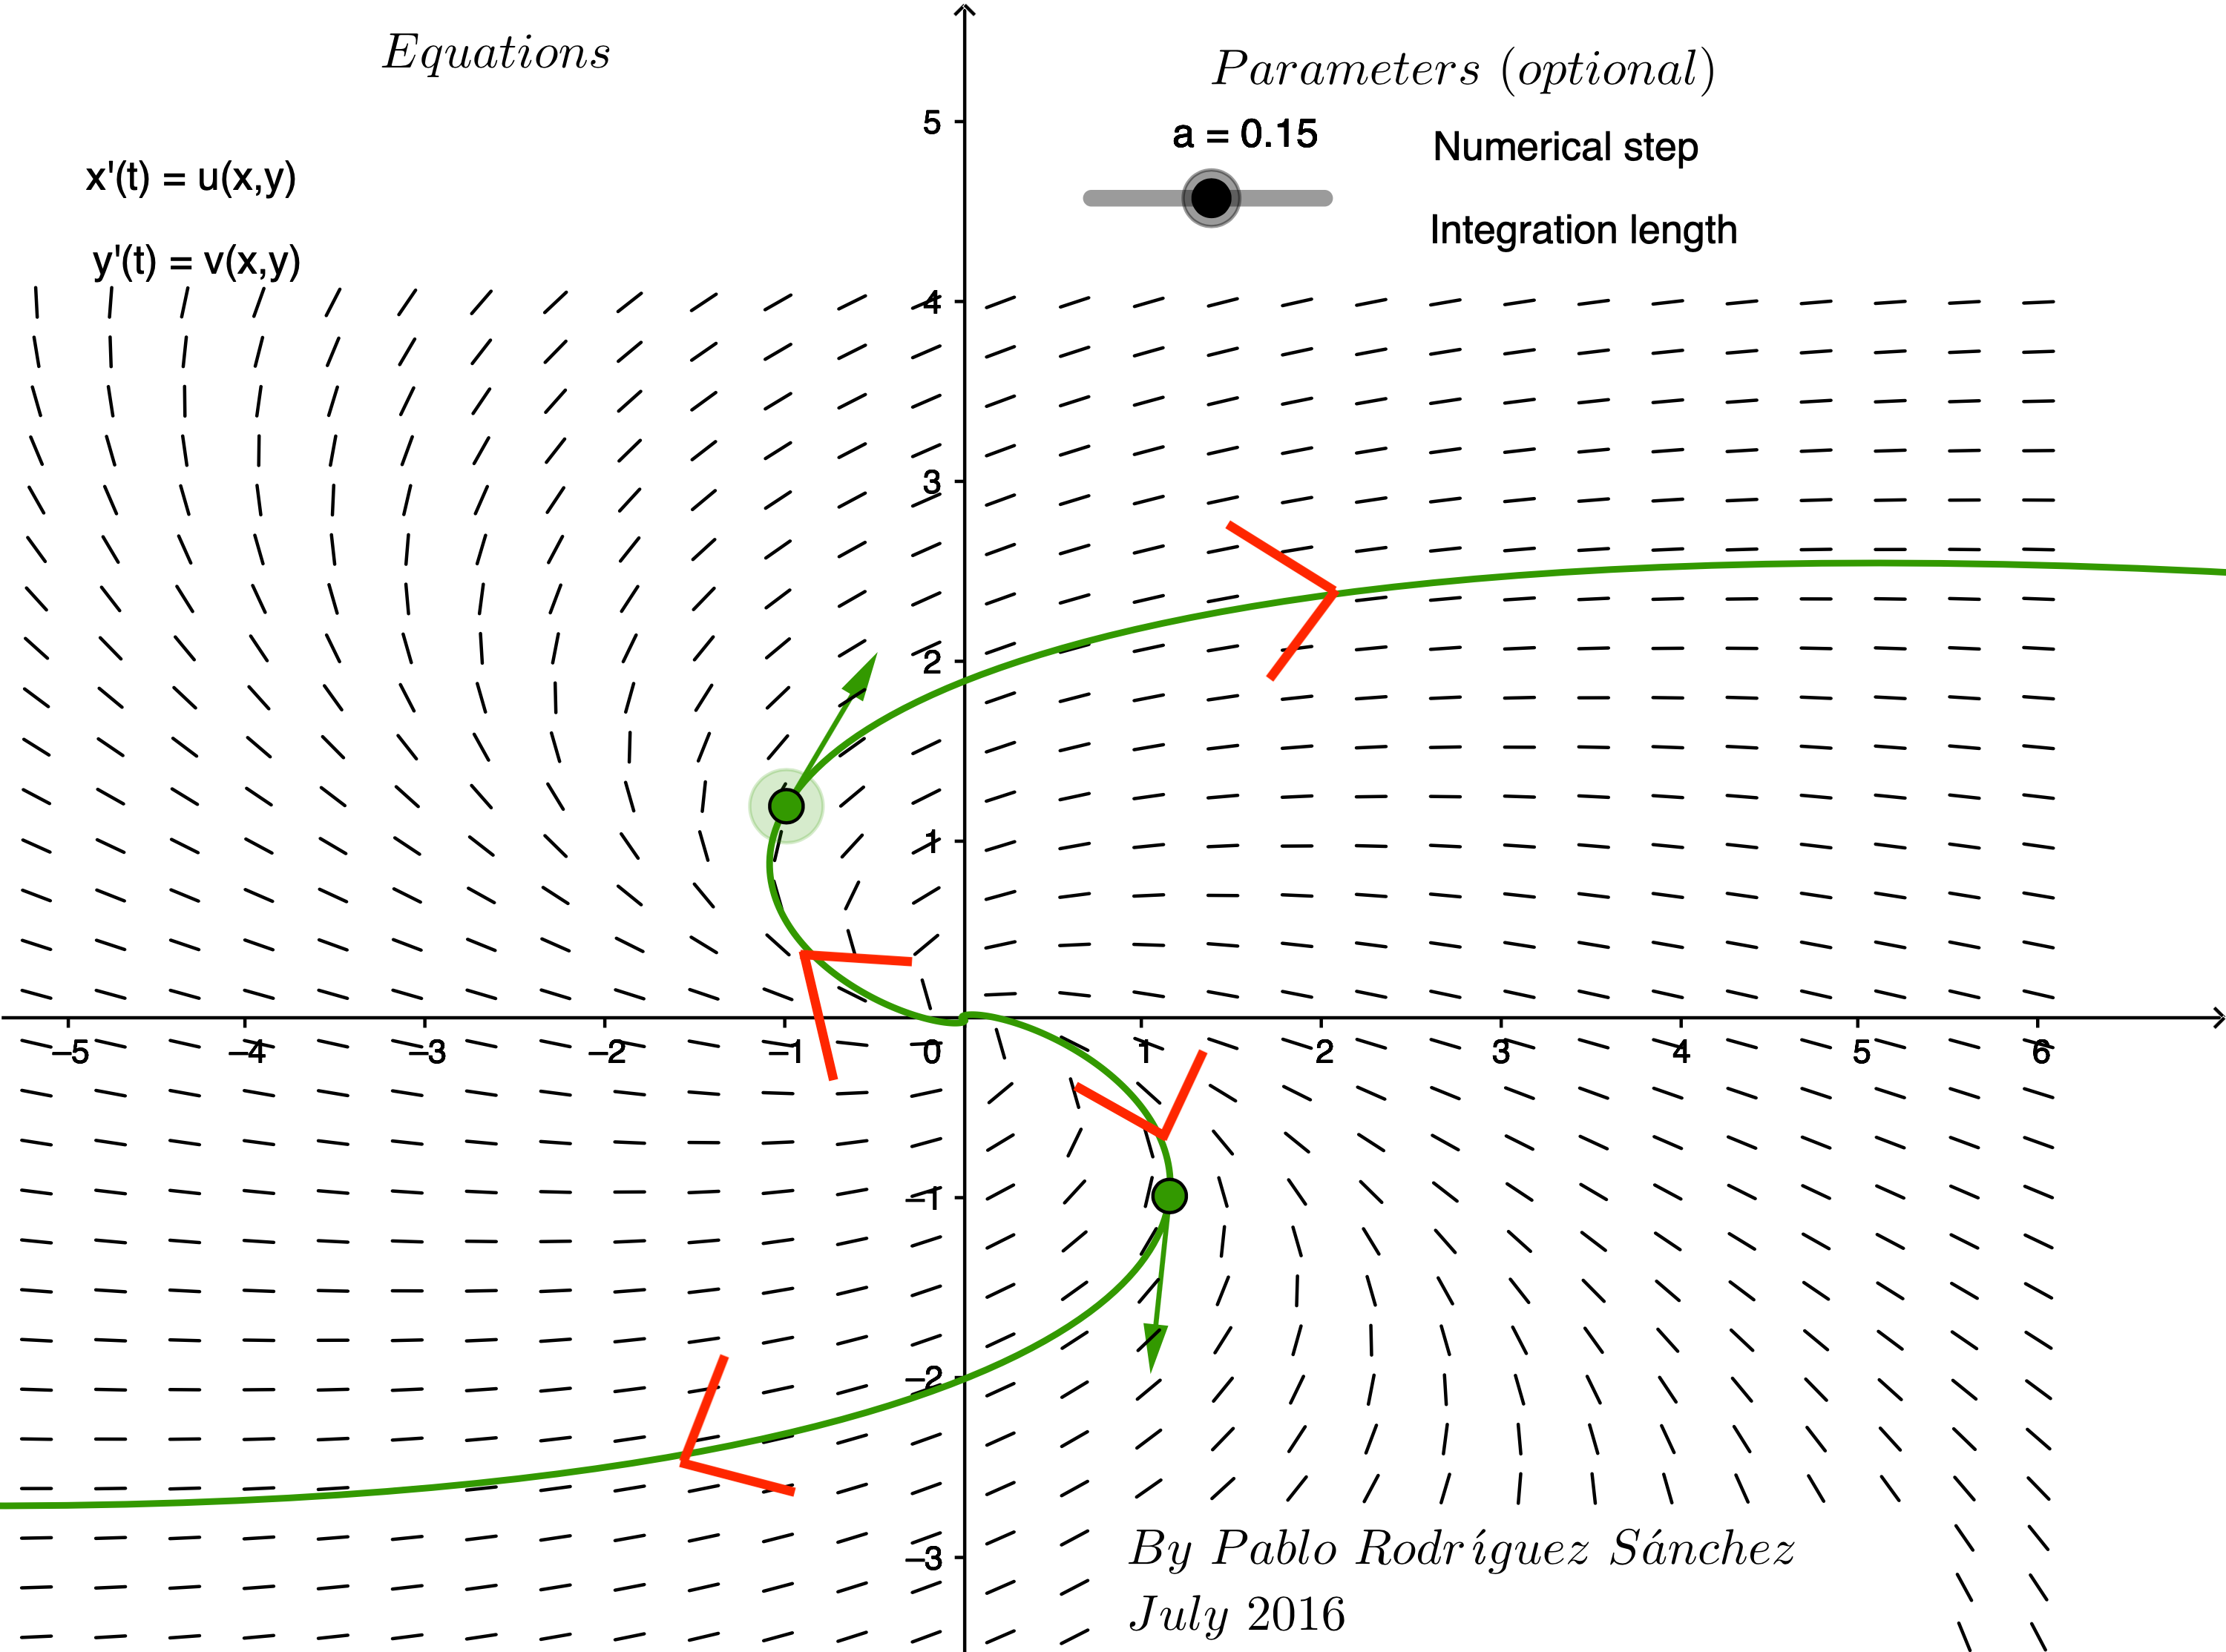
\includegraphics[width=0.45\tw]{14/14-complex-pos.png} &
F. 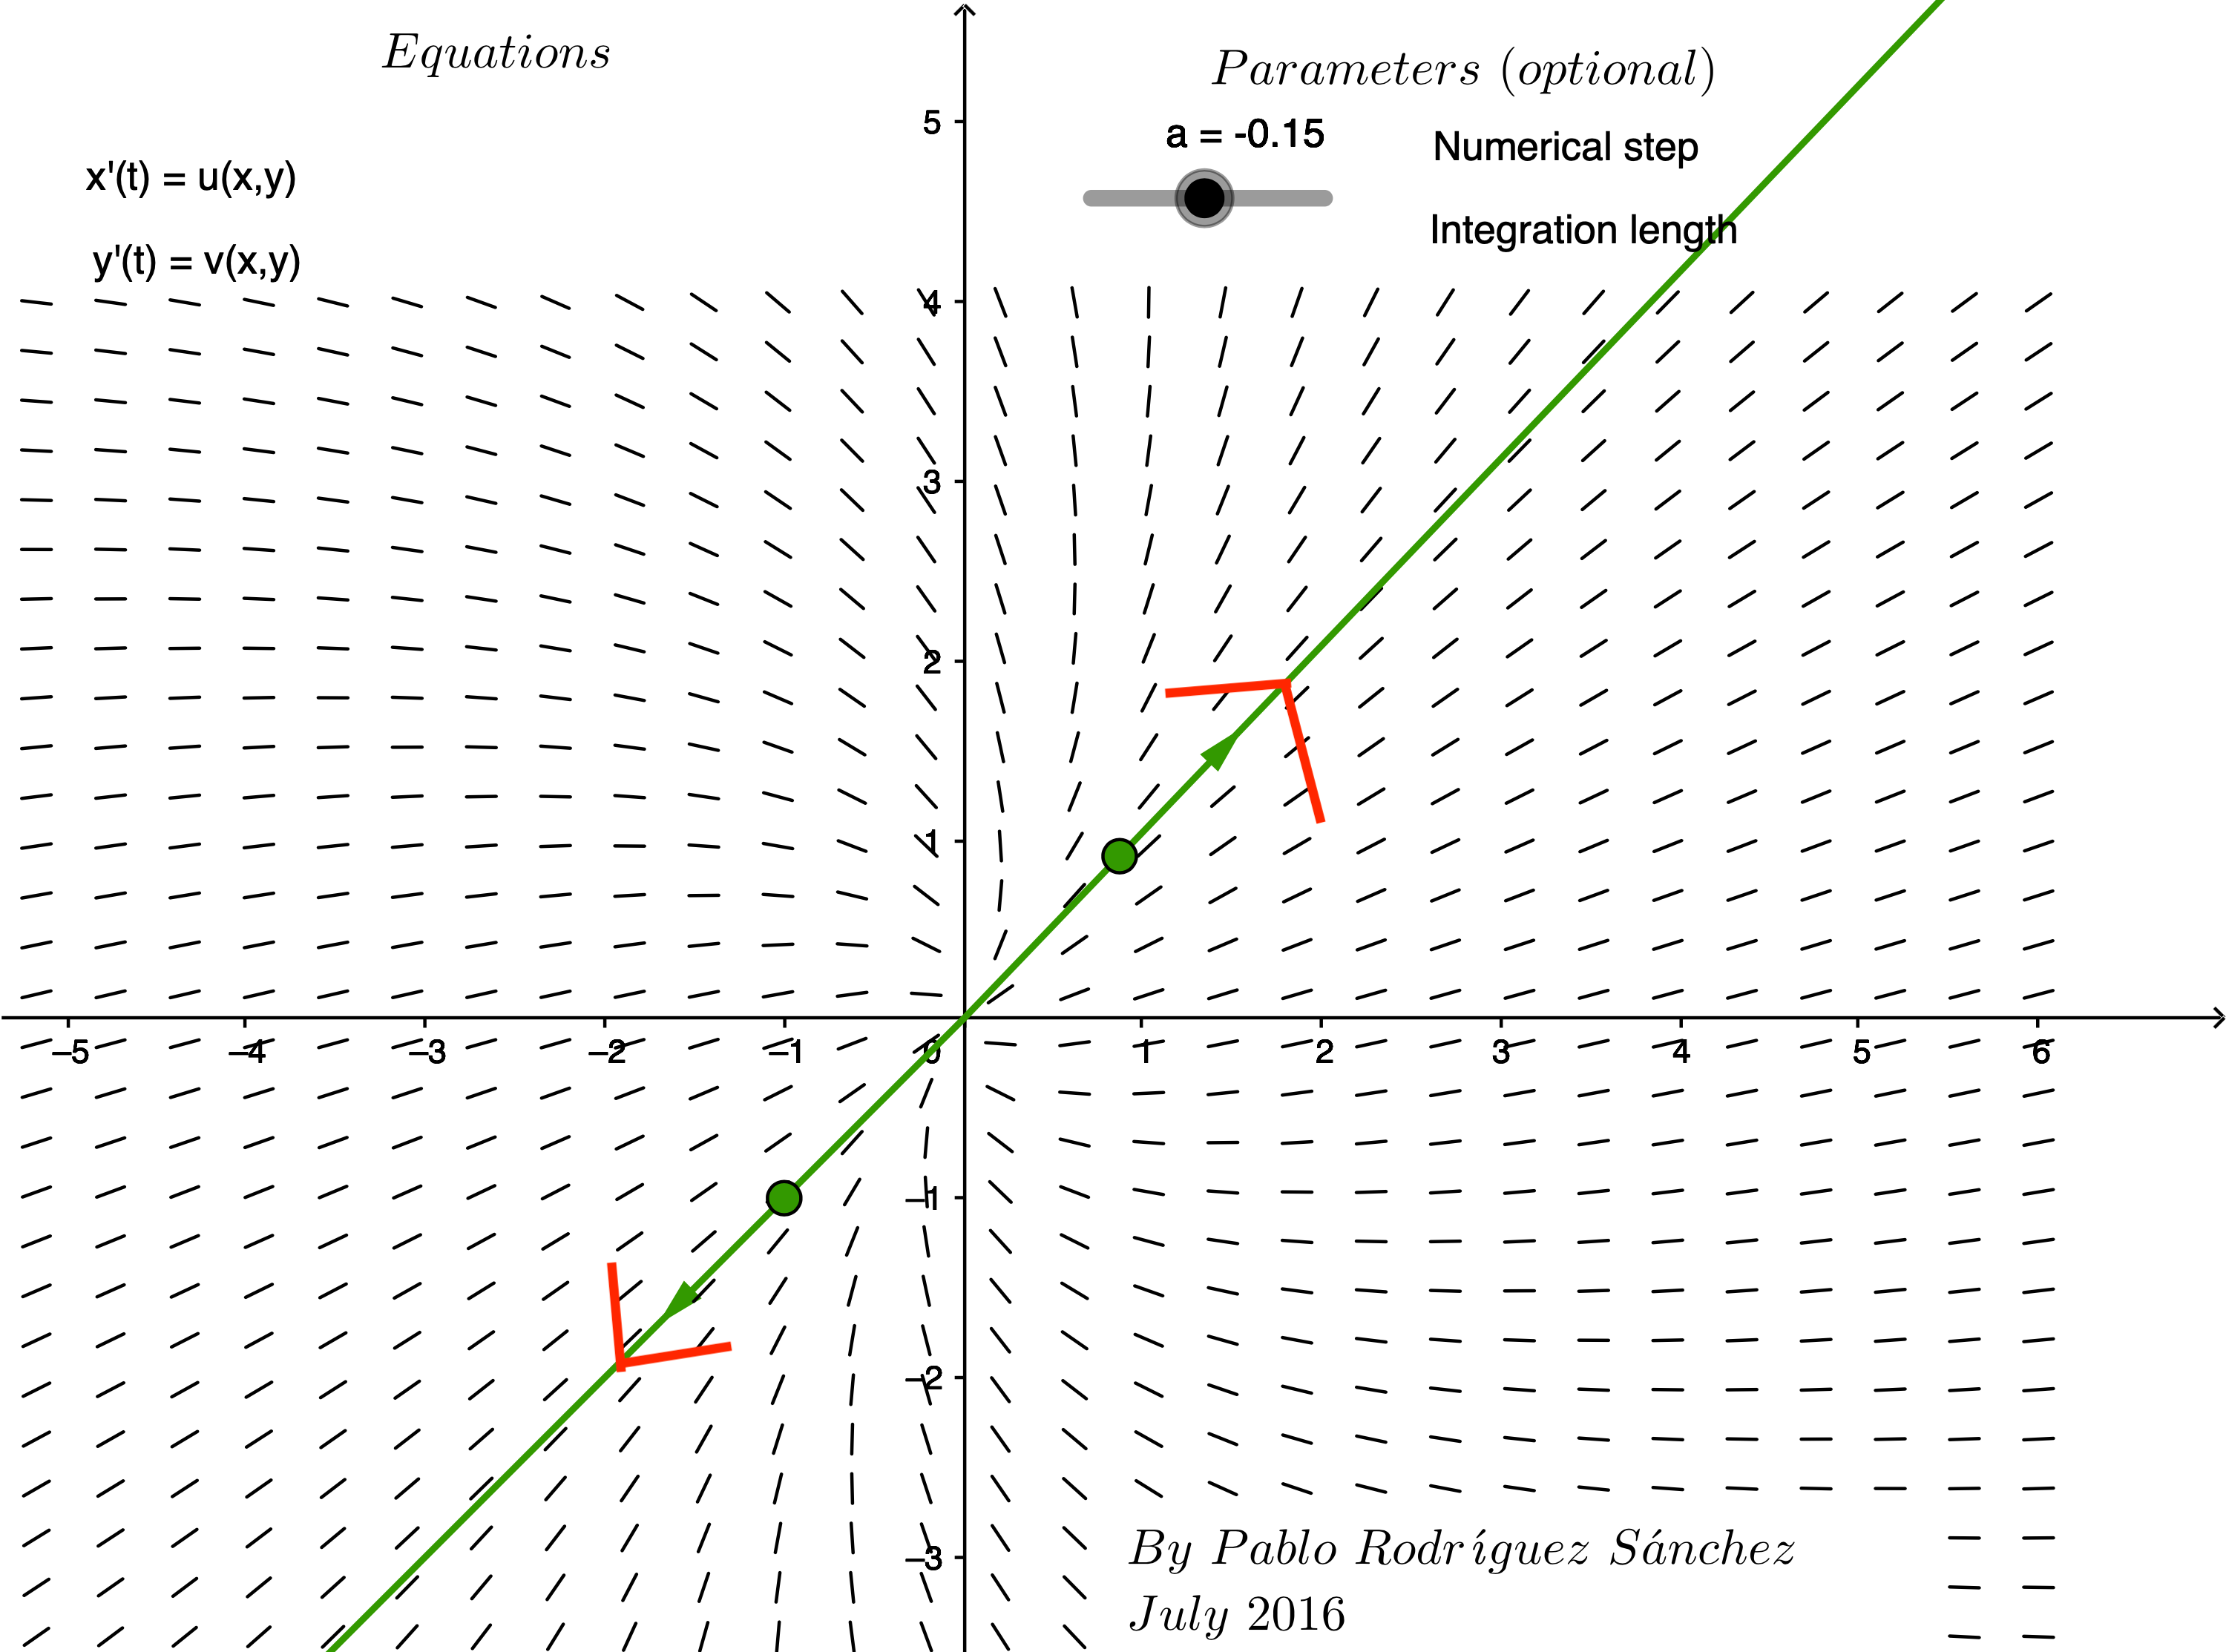
\includegraphics[width=0.45\tw]{14/14-repeated-pos.png} \\
\hline
\end{tabular}


\clearpage

\pagebegin{Stability of the Equilibrium}

\ii Based on your answers in problem \ref{14problem6}, explain how the eigenvalues can be used to determine whether the equilibrium at the origin is stable or unstable?  What happens when the matrix of coefficients has complex eigenvalues?\label{14problem7} 

\vfill

\ee

%\clearpage

%\pagebegin{Extra Practice}

%\ii Find and sketch several solutions in the phase plane for each of the systems below.
%\bb
%\ii $\dsty \begin{array}{l} x'=-\frac{20}{9}x-\frac{8}{9}y\\ y'=-\frac{4}{9}x-\frac{34}{9}y\end{array}$ \vfill %real -4 and -2 with v1=<1,2> and v2 = <-4,1>
%\ii $\dsty \begin{array}{l} x'=x-y\\ y'=2x-y\end{array}$ \vfill %Pure imag with \pm i with v1=<1+i,2> and v2=<1-i,2>
%\ii $\dsty \begin{array}{l}x'=12x-3y\\y'=3x+6y \end{array}$  \vfill %Repeated 9 v=<1,1>

%\clearpage

%\ii $\dsty \begin{array}{l} x' =4x+5y\\y'=-x+2y \end{array}$ \vfill %Imag with 3 \pm 2i and v1=<-1-2i,1> and v2=<-1+2i,1>
%\ii $\dsty \begin{array}{l} x'=4x+21y\\y'=-2x-8y\end{array}$ \vfill %Imag with -2 \pm i\sqrt{6} and v1=<-6-i\sqrt{6},1> and v2=<-6+i\sqrt{6},1>
%\ii $\dsty \begin{array}{l} x'=2x+2y\\y'=x+3y \end{array}$ \vfill %real 4 and 1 with v1=<1,1> and v2=<-2,1>%\

%\ee

